\documentclass[final]{cmpreport}
\usepackage{comment}
\graphicspath{ {./images/} }

\title{GPU Accelerated Method for Constructing and Rendering Trees}
\author{Thomas Mcloughlin}
\date{21/3/2021}
\registration{100203952}
\ccode{CMP - 6013Y}
\supervisor{Dr. Stephen Laycock}

\summary
{
This project aims to convert and extend the Lindenmayer-system based tree construction 
method presented by \citep{prusinkiewicz1996systems} to be used as an independent 
OpenGL module. 
The module should allow the addition of trees to a real-time environment with minimal 
user interaction, avoiding the difficulties and expenses of manually producing tree 
models.
}

\acknowledgements
{
I'd like to thank my supervisor, Stephen Laycock for his brilliant help and support 
throughout this project.
Thank you to George Smith and Harry Tucker for their interest in my work and their 
support during the COVID-19 lockdowns. 
}

\begin{document}

\section{Introduction}
In this section a context will be provided for the 

\subsection{Context}
Creating and rendering realistic models of trees manually requires advanced expertise 
with modelling software packages. This limits the ability to produce convincing 3D 
scenes for small developers with restricted resources.

The purpose of including trees in a natural environment is to provide realism. 
Trees are common natural structures present in even simple environments 
throughout the history of computer graphics and have seen many iterations as 
technology has advanced allowing for more detailed and realistic results.

The aim of this project is to provide a method for creating and rendering trees 
to be used in a real-time graphics application. This method should be simple to 
use and implement into an existing OpenGL project.

\subsection{Related Work}
In this subsection various related works will be discussed with respect to how they 
contribute to the main knowledge required for this project, ordered chronologically. 
These areas of main knowledge are the branching structure, branch thickness and leaf 
placement of the constructed trees.

A paper by \cite{lindenmayer1968mathematical} proposes a theory for the development 
of organisms using a cells current state and being combined with input that the cell 
receives from its neighbour. Two new cells are produced from this development to replace 
the existing cell and the cycle repeats for the two new cells. 

This process of generating new outputs recursively to produce larger structures became
``Lindenmayer systems'' or the abbreviated ``L-systems'' which became important tools 
in pattern generation for future applications. L-systems became a common approach for the 
generation of branching patterns in flora which is where the aim of this project is 
concerned.

Another early paper that is referenced by many later studies of the subject is by
\cite{honda1971description} where he presented one of the earliest algorithmic 
methods for creating a branching structure. This was done by starting with a parent 
branch which then bifurcates into two child branches and rotating them by given 
angles about the termination point of the parent branch, an example of which 
can be seen in Figure \ref{fig:honda-bifurcation}. By continuing this 
method he treated each child branch as another parent and bifuracted them to 
expand the branching structure which would be continued until a desired result is 
reached.

\begin{figure}[ht]
    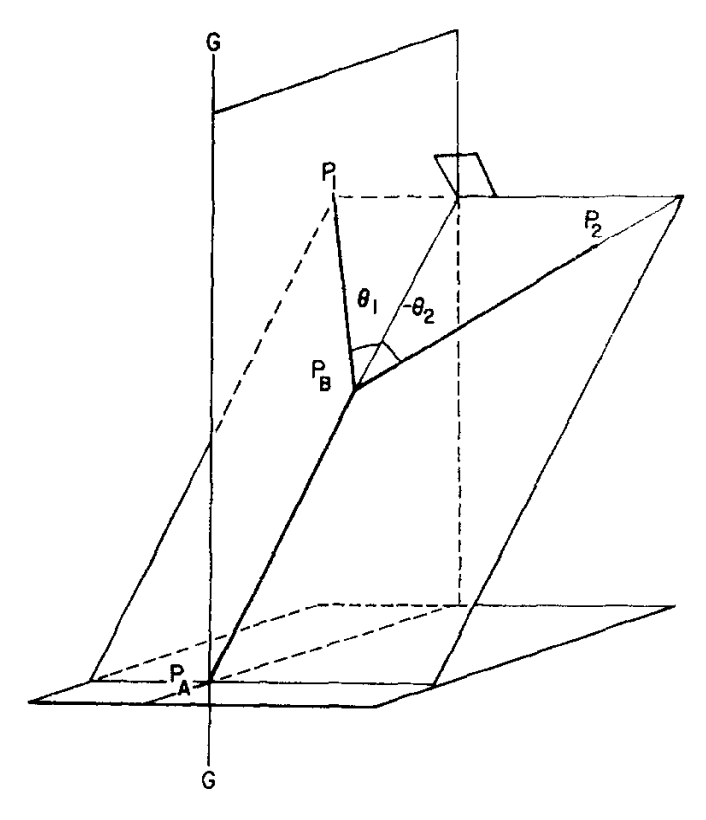
\includegraphics[scale=0.5]{honda-bifurcation.PNG}
    \centering
    \captionsetup{justification=centering}
    \caption{Example diagram of parent branch $P_AP_B$ bifurcating into child branches
    $P_BP_1$ with a rotation of $\theta_1$ and $P_BP_2$ with a rotation of \textminus$\theta_2$}
    \label{fig:honda-bifurcation}
\end{figure}

This paper does not include any information relating to branch thickness or leaf 
placement as its focus was only on the branching structure. However, this paper 
provides a groundwork for many later studies that will be discussed in this project.

\cite{bloomenthal1985modeling} presents his own tree generation process, specifically 
for a maple tree. For the construction of the branches and 
trunk he uses splines to create a tree skeleton, the use of splines rather than 
straight lines is chosen to produce a more natural structure. He then uses generalised 
cylinders with varying radii across the splines to create thickness. He also describes 
the use of ramiforms, shown in Figure \ref{fig:bloomenthal-ramiform}, to make branch 
bifurcations realisticly curve rather than have an acute separation.

\begin{figure}[ht]
    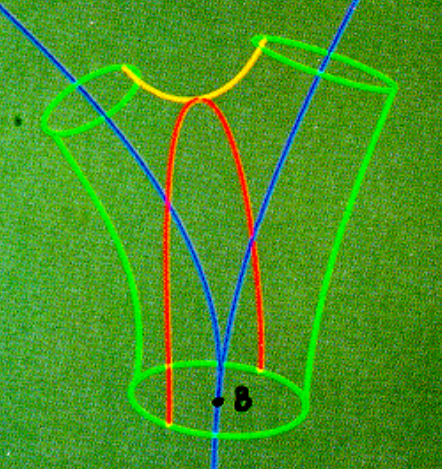
\includegraphics[scale=0.6]{bloomenthal-ramiform.PNG}
    \centering
    \captionsetup{justification=centering}
    \caption{A ramiform used to create a realistic bifurcation}
    \label{fig:bloomenthal-ramiform}
\end{figure}

The method he describes for leaf placement uses polygon structures to which he applies 
a leaf texture, these polygons are then brought together in clusters that he calls 
``configurations'' and for each limb that does not exceed a given diameter and that has 
no outgoing limbs, a leaf configuration is chosen at random, scaled randomly and placed 
at the limb tip. The interior lines of each polygon correspond to hinge points of the 
leaves that could be manipulated to show leaf distortion from wind. 

\begin{figure}[ht]
    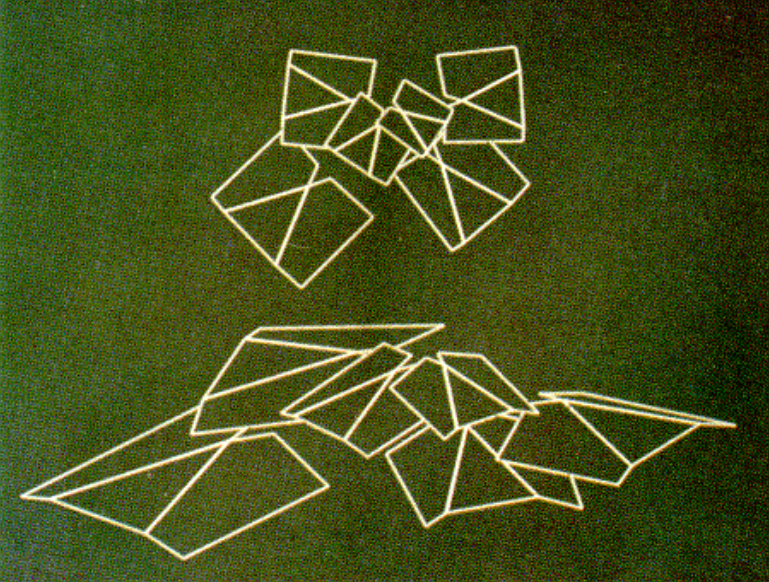
\includegraphics[scale=0.35]{bloomenthal-leaves.PNG} 
    \centering
    \captionsetup{justification=centering}
    \caption{A leaf configuration: plan view (top) and perspective view (bottom)}
    \label{fig:bloomenthal-leaves}
\end{figure}



\cite{prusinkiewicz1996systems} presents a method of tree generation using an advanced 
L-system, developed from the work of \cite{lindenmayer1968mathematical} and applying 
that system to the bifurcating parent and child branch trios displayed by \cite{honda1971description}.
Their chosen method for representing their models is by using turtle graphics in a 3D 
space and the string generated from the L-system uses symbols that correspond to controlling 
the turtles orientation in space.

Prusinkiewicz et al. produce a variation on a standard L-system known as a ``deterministic''
L-system or ``D0L-system'' which produces the same result every time. They demonstrate the 
application to turtle graphics with a simple snowflake fractal shown in Figure \ref{fig:snowflake-lsystem}.

The D0L-system uses an Axiom string and a production rule to recursively develop a longer and 
more complex string. Once a chosen result is reached, the string is traversed and each character 
or group of characters corresponds to the movement of the turtle. For example the D0L-system 
below represents that of the snowflake fractal where $F(s)$ corresponds to a movement forward 
of distance $s$ and $+(r)$ or $-(r)$ correspond to a rotation positively or negatively about the
$x$ axis by $r$ degrees.

\textbf{Axiom} $\omega$: $F(1) - (120)F(1) - (120)F(1)$ 

\indent \textbf{Production} $p_1$: $F(s) \rightarrow F(s/3) + (60)F(s/3) - (120)F(s/3) + (60)F(s/3)$

The axiom draws an equilateral triangle with edges of unit length. Production $p_1$ replaces 
each line segment with a polygonal shape where the line segment has been given a convex 
triangular appendage. The Production $p_1$ can be visualised as so:

\begin{figure}[ht]
        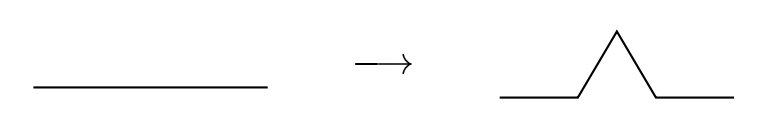
\includegraphics[scale=0.4]{production_p1.PNG}
        \centering
        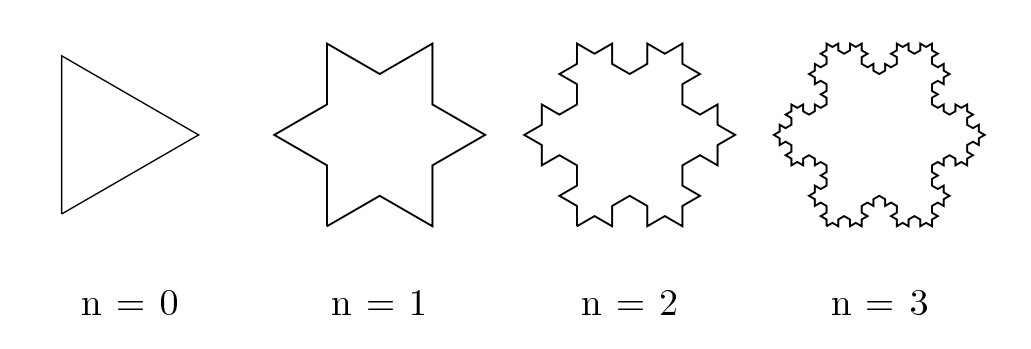
\includegraphics[scale=0.5]{triangle_snowflake_lsystem.PNG}
        \centering
        \caption{The visualised production rule $p_1$, axiom and first 3 recursions 
        defined by the snowflake D0L-system from \citep{prusinkiewicz1996systems} pg.12}
        \label{fig:snowflake-lsystem}
\end{figure}

Prusinkiewicz et al. went on to present a complex D0L-system to be used for constructing 
tree structures by creating a Parametric L-system allowing for input to alter the axiom 
string producing different results along with using a conditional requirement to 
decide automatically when to stop recursing. 

This L-system is defined below, in this 
context $A(s, w)$ refers to a line segment or ``apex'' of length $s$ and width $w$. 
Production $p_1$ begins with the conditional statement to only continue if the length $s$ 
of the current apex is greater than or equal to $min$ which is a chosen minimum length. If 
the condition is met then $!(w)F(s)$ draws a line of length $s$ and width $w$. 

Lines $a_1$ and $a_2$ refer to the bifurcated child apices of the parent apex which are 
given a rotation of $\alpha_1$ and $\alpha_2$ radians about the $x$ axis and a rotation of 
$\phi_1$ and $\phi_2$ radians about the $y$ axis. The length of the child apices is calculated 
by multiplying the parent apex length $s$ by the corresponding length degradation parameters 
$r_1$ and $r_2$ respectively. A degradation in width is calculated using $q$ and $e$.

\begin{comment}
$\omega$: $A(100, w_0)$ 

\indent $p_1$: $A(s, w) : s >= min \rightarrow !(w)F(s)$

\indent $a_1$ $[+(\alpha_1)/(\phi_1)A(s * r_1, w * q ^ e)]$

\indent $a_2$ $[+(\alpha_2)/(\phi_2)A(s * r_2, w * (1 - q) ^ e)]$
\end{comment}

\begin{figure}[ht]
    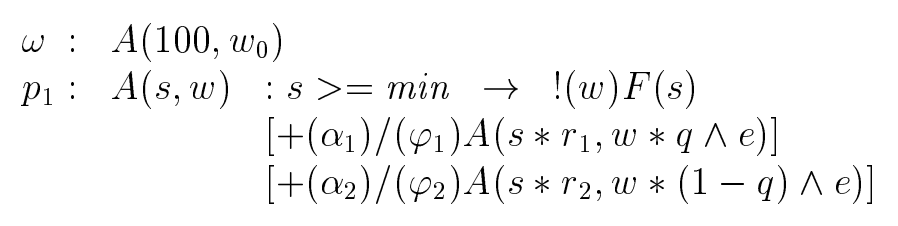
\includegraphics[scale=0.5]{parameterised-tree-lsystem.PNG} 
    \centering
    \captionsetup{justification=centering}
    \caption{Parameterised Tree L-system}
    \label{fig:parameterised-tree-lsystem}
\end{figure}

This L-system is used to produce various complex tree patterns, shown in section 
\ref{app:parameterised-lsystem-trees} of the Appendix, ranging from mathematical fractal 
patterns to some realistic looking structures.

Prusinkiewicz et al. do not directly propose a method of leaf placement as this 
paper focuses on tree structure and the manipulation of L-systems, they do however provide 
an example where terminating apices of an L-system could be replaced with a leaf shape to 
give a rudimentary leaf placement approach.



%Bibliography
\bibliography{bibfile}

%Appendix
\appendix{}
\begin{figure}[ht]
    \section{Parameterised L-system Trees}
    \label{app:parameterised-lsystem-trees}
    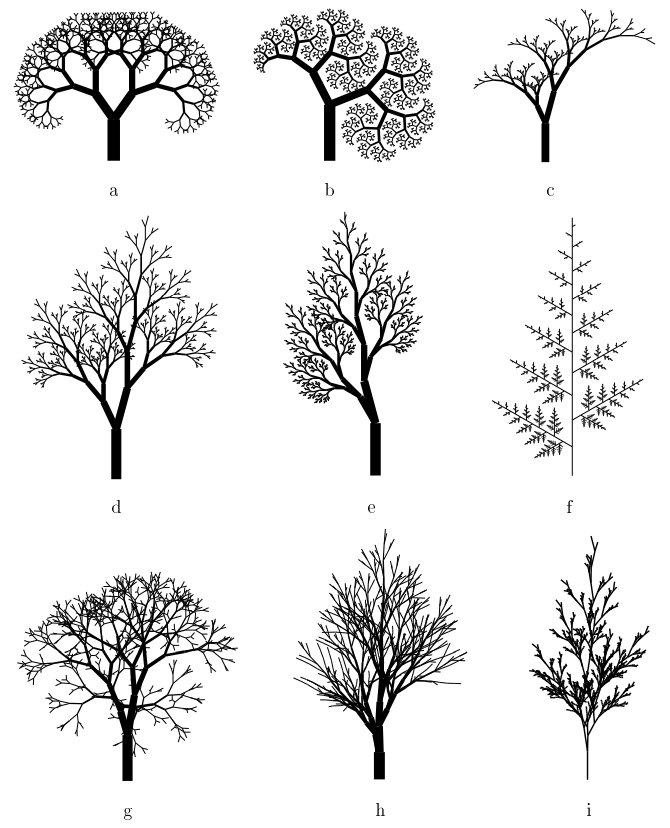
\includegraphics[scale=0.7]{tree-lsystem-results.PNG} 
    \centering
    \captionsetup{justification=centering}
    \caption{Tree structures produced using the proposed L-system described by \cite{prusinkiewicz1996systems}}
    \label{fig:tree-lsystem-results}
\end{figure}

\end{document}